\chapter{Wissensrepräsentationsformen}
\label{chap:wissensrepFormen}

Nach Darstellung der Grundlage von Graphen und Graphdatenbanken im letzten Kapitel, wollen wir jetzt Repräsentationsformen von Wissen analysieren.\\
In der Wissensmodellierung (knowledge engineering) gibt es verschiedene Formen der Wissensrepräsentation um Wissen in wissensbasierten Systemen formal abzubilden. Auf diese Art abgelegte Informationen werden als Wissensdatenbank bzw. Wissensbasis bezeichnet.~\cite{wikiWissensrep}

Das folgende Kapitel basiert auf~\cite{laemmel} und beschreibt einige klassische Formen der Wissensrepräsentation, nämlich semantische Netze, Wissensnetze und Frames.

Im Gegensatz zu Regeln stehen hier die Objekte und nicht Zusammenhänge und logische Abhängigkeiten im Vordergrund.

Semantische Netze und Frames versuchen das menschliche Gedächtnis abzubilden. Sie wurden hauptsächlich zur Analyse von Wörtern und Sätzen verwendet. Ein weiterer Aspekt ist die verständliche Darstellung von Klassen und ihren Beziehungen. Die Konzepte der semantischen Netze und Frames haben die Entwicklung der objektorientierten Programmierung beeinflusst.

\section{Semantische Netze}
\label{sec:wissensrepFormen_semantischeNetze}

Eine zusammengehörige Gruppe von Objekten wird als Klasse bezeichnet. Ein einzelnes Objekt heisst Individuum. Es gibt Beziehungen zwischen Objekten, zwischen Objekten und Klassen und zwischen Klassen.

Folgende Beziehungen werden unterschieden:
\begin{itemize}
    \item ``ist ein'' Relation

        Es handelt sich um Ober- und Unterklassen.

        Beispiel: \textit{Ein Baum ist eine Pflanze.}

    \item ``Instanz von'' Relation

        Die Relation sagt aus von welchem Typ ein Individum ist.

        Beispiel: \textit{Birke ist eine Instanz der Klasse Baum.}

    \item Eigenschaft

        Klassen und Objekte haben Eigenschaften.

        Beispiel: \textit{Pflanzen erzeugen Sauerstoff.}
\end{itemize}

Eigenschaften sind transitiv: Ist also ein Hund ein Tier und ein Tier ein Lebewesen, ist auch ein Hund ein Lebewesen. Weiter unterliegen Eigenschaften de, Gesetz der Vererbung. Ein Tier benötigt Sauerstoff, damit benötigt auch ein Hund Sauerstoff.

In semantischen Netzen werden Objekte und Klassen als Knoten abgebildet. Beziehungen und Eigenschaften werden als Kanten dargestellt.
Aussagen wie Existenzaussagen und Oder-Aussagen können mit semantischen Netzen nicht abgebildet werden.
Komplexe Abbildungen, wie zum Beispiel das Modellieren einer Aktion, sind trotz reinen zweistelligen Beziehungen möglich.

\section{Frames}
\label{sec:wissensrepFormen_frames}

In Frames werden die wesentlichen Charakteristika eines Objektes als Eigenschaften abgebildet. Dabei unterstützen Frames die Konzepte der Hierarchie und der Vererbung. Frames können auch generische Informationen wie Standartwerte (Defaults) und Wertebeschränkungen (Listen) enthalten.

\begin{lstlisting}[caption={Beispiel eines Frames anhand einer Reise.}]
    frame Abenteuerreise is a Reise :
        default hatReiseleiter is true
    instance `Dschungeltrip' is a kind of Abenteuerreise :
        anbieter is dernettereiseanbieter
        and typ is abenteuer
        and kosten is 1000.
    constraint preise
        when the typ of an Abenteuerreise changes to X
        then check that X is {dschungel or abenteuer or nevernkitzel or natur}
        otherwise write( `Der Typ der Reise wurde nicht geändert' )
        and nl.
\end{lstlisting}

\section{Wissensnetze}
\label{sec:wissensrepFormen_Wissensnetze}
Bei Wissensnetzen handelt es sich um eine bestimmte Art der Wissensrepräsentation. Dabei werden die Konzepte der semantischen Netze verwendet.

Wissen wird in Wissensnetzen objektorientiert oder mittels Frames abgebildet. Eine grafische Darstellung erfolgt zusätzlich mittels Topic Maps, auch Wissenslandkarte genannt.

``In einer Wissenslandkarte repräsentiert die Entfernung zweier Begriffe oder Wissensinhalte deren inhaltliche Nähe zueinander. Ein Wissensnetz ist somit ein Informationssystem, in dem zusätzlich die semantischen Beziehungen der Begriffe untereinander verwaltet werden. Diese Meta-Ebene ermöglicht eine \textbf{semantische Suche} – eine Suche, die über das Auffinden reiner Zeichenketten weit hinausgeht.''~\cite[S. 89]{laemmel}.

Die Knoten erhalten die Bedeutung von Instanzen (Individuen) oder Klassen. Das Problem der Mehrfachvererbung durch Einführung des Rollenkonzeptes umgangen. Durch Erweiterung der Klassen kann eine Instanz dann eine bestimmte Rolle einnehmen.

Wissensnetze haben alle Voraussetzungen, um effektives Wissensmanagement zu bieten. Dafür muss das Wissen aber immer aktuell und umfassend sein.

\newpage

\noindent\rule[1ex]{\textwidth}{1pt}
\begin{wrapfigure}[9]{l}{0.1\textwidth}
    \vspace{-2pt}
    
\includegraphics[width=0.1\textwidth]{bilder/owl.png}
\end{wrapfigure}\\
Ein sehr wichtiger und zeitintensiver Teil des Knowledge Engineerings ist die tatsächliche Modellierung. Also die Überlegung ob eine abzubildende Information ein Objekt, eine Instanz oder eine Eigenschaft ist, oder, ob sie gar als Regel abgebildet werden kann. Regeln werden im Kapitel~\ref{chap:swrl} \nameref{chap:swrl} genauer erläutert. Uns scheint an dieser Stelle aber wichtig zu erwähnen, dass das semantischen Netz ein sehr gutes Hilfsmittel war, um einen Überblick über die Informationen und ihre Verwendbarkeit zu erhalten. Würde man das Wissen direkt in die semantische Datenbank übertragen, wäre diese nicht viel mächtiger als eine traditionelle Wissensspeicherung. Dies führen wir zu einem späteren Zeitpunkt noch genauer aus.

\noindent\rule[1ex]{\textwidth}{1pt}


\noindent\rule[1ex]{\textwidth}{1pt}
\begin{wrapfigure}[6]{l}{0.1\textwidth}
    \vspace{-12pt}
    
\includegraphics[width=0.1\textwidth]{bilder/elephant.png}
\end{wrapfigure}
Möchte man nun ein semantisches Netz als Hilfsmittel zur Aufbau der Ontologie für einen Reiseplaner nutzen, so ist das Vorgehen dem der Graphdatenbank sehr ähnlich. 

Gegeben sind nach wie vor die zuvor gemachten Überlegungen zum Aufbau, also auch die Klassen, Individuen und deren Relationen. Aktuell sind dies die Klassen \textit{Ausflug}, \textit{Land}, \textit{Region} und \textit{Ort}, die Individuen \textit{Schweiz}, \textit{Solothurn}, \textit{Bern} und \textit{Seilpark Balmberg} sowie die Relationen \textit{hatRegion} und \textit{hatOrt}.

Doch wie geht man nun weiter vor? Was unterscheidet denn ein semantisches Netz eigentlich von einer Graphdatenbank? Nun, im Kapitel zu den Graphdatenbanken wurde bereits eine wichtige Entität vorweggenommen, welche einer Hauptunterschiede zwischen einem semantischen Netz und einer Graphdatenbank darstellt: die Individuen. Diese lassen sich in Graphdatenbanken zwar abbilden, aber viel weniger intuitiv und sinngemäss.

An diese Stelle läuft man jedoch schnell in Gefahr, eine ähnliche Modellierung wie bei der Graphdatenbank zu erhalten. Wir haben uns daher bei der Modellierung an den Aufbau der letztendlich verwendeten Ontologiesprache OWL 2 bzw.\ deren Anwendung im Editor Protégé der Universität Stanford gehalten, da wir das Gefühl haben, dass dies einen guten Rahmen vorgibt.

Schlussendlich ist ja das Ziel, die bereits formulierten Kriterien, \textit{familienfreundlich}, \textit{regional} und \textit{actionreich}, abzubilden, um letztendlich entsprechende Abfragen stellen zu können. Unter den gegebenen Entitäten scheint sich aktuell nur das Kriterium \textit{regional} abzubilden lassen, doch wie setzt man dies nun um? Davon ausgehend, dass der Standort bzw.\ die Region der Familie bekannt ist --- diese sei der Einfachheit halber Solothurn ---, sollte es also möglich sein, zu Folgern, dass die Region des Seilparks Balmberg dieselbe wie die der Familie ist.

Man kann nun also mittels der Relation \textit{hatOrt} definieren, dass die \textit{Region} \textit{Solothurn} den \textit{Ort} \textit{Balmberg} hat. Dies lässt jedoch noch keinen Schluss zu, dass sich der Seilpark Balmberg im selben \textit{Ort}, ja, sogar in derselben \textit{Region} befindet. Es scheint eine Relation zu fehlen. Dies führt zur Einführung der neuen Relation \textit{hatStandort}, welche das Individium \textit{Seilpark Balmberg} mit dem Ort \textit{Balmberg} verbindet.

\newpage

Das oben Genannte könnte folgendermassen aussehen:

\begin{figure}[H]
\centering \rotatebox{0}{\scalebox{0.5}[0.5]{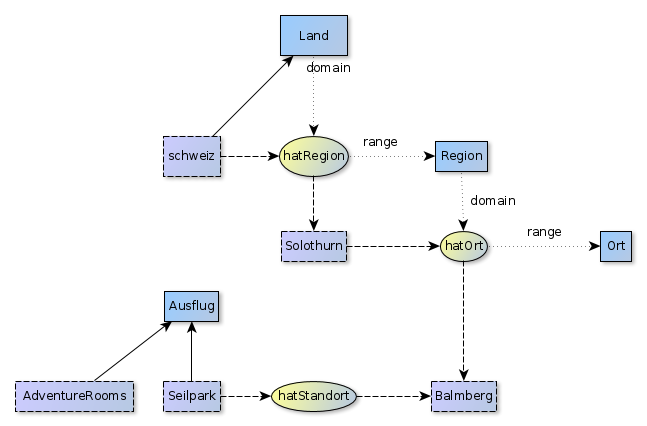
\includegraphics{bilder/beispiel_semantisches_netz.png}}}
\caption{Abbildung von Wissen mittels einem semantischen Netz.\label{fig:semantischesNetz}\protect\footnotemark}
\end{figure}
\footnotetext{Eigene Darstellung mittels yEd}

Die obige Abbildung mag auf den ersten Blick simpel erscheinen, wie aber bereits vorher erwähnt, handelt es sich um einen Übersicht der Informationen. 

Wie gelangt man nun aber zum Schluss, dass das Individuum \textit{Seilpark Balmberg} die \textit{Region} \textit{Solothurn} hat? Dies scheint sich aus dem gegebenen semantischen Netz nicht folgern zu lassen. Wir stellen fest, dass die Möglichkeit der Folgerung aktuell fehlt.

\vspace{0.1pt}
\noindent\rule[1ex]{\textwidth}{1pt}

% Einträge im Verzeichnis erscheinen lassen ohne hier eine Referenz einzufügen
%\nocite{kopka:band1}
